

\section{prova}
questa prova include tutte le note del video introduttivo\footnote{a partire dalle footnote}

\subsection{banco di prova}\label{sec: banco di prova}
in questa sezione si parla della Progettazione di un banco prova per strumenti endodontici(\ref{sec: analisi fem}) - Progetto di un banco prova per la sperimentazione di strumenti endodontici per il trattamento di canali reticolari, sottoposti a carichi combinati di fatica flessionale, di torsione statica e di usura.\cite{}

\subsection{analisi fem}\label{sec: analisi fem}
in questa sezione si discute del fatto che come visto durante la progettazione si è analizzato l'analisi fem
\begin{equation}
    x=\frac{2}{3} \lambda
\end{equation}

\begin{table}
    \centering
    \begin{tabular}{c|c}
         &  \\
         & 
    \end{tabular}
    \caption{tabella di esempio}
    \label{tab:placeholder}
\end{table}

\begin{figure}
    \centering
    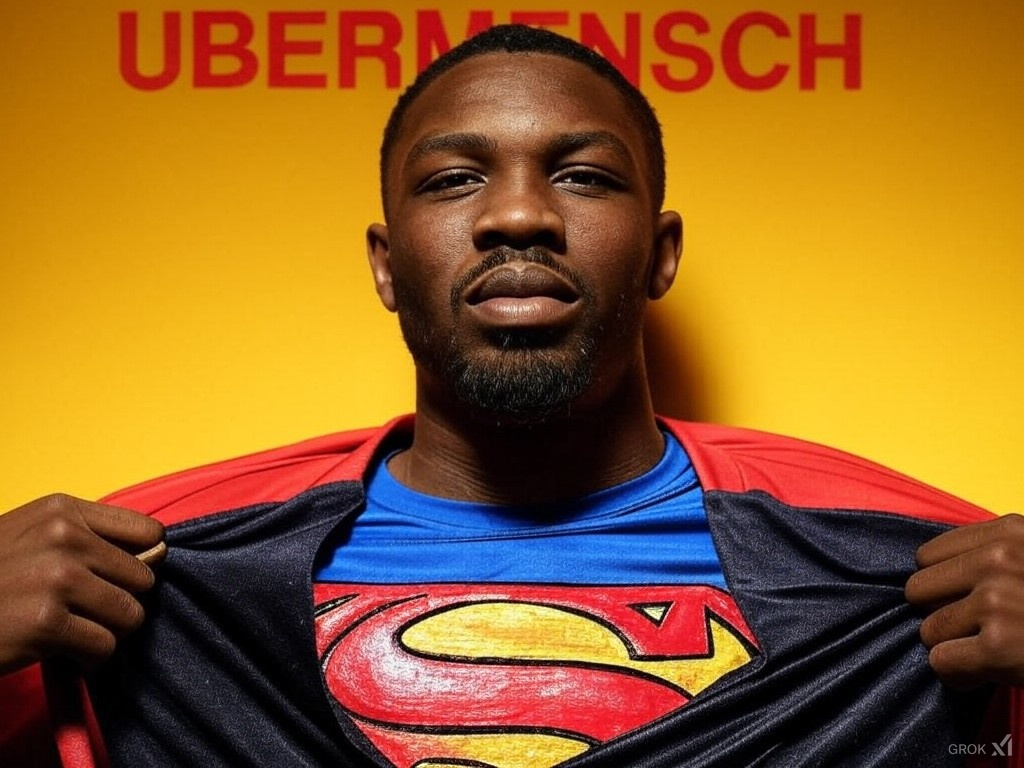
\includegraphics[width=0.5\linewidth]{images/uber.jpg}
    \caption{uber}
    \label{fig:placeholder}
\end{figure}
